\documentclass[12pt]{article}

\usepackage{sbc-template}
\usepackage[utf8]{inputenc}
\usepackage[T1]{fontenc}
\usepackage{graphicx,url}
\usepackage{booktabs}
\usepackage{tikz}
\usetikzlibrary{arrows.meta}

\sloppy

\title{A Verified Five-Stage Pipelined RV32E Core in Verilog}

\author{Lucas dos Anjos Camelo, João Vitor Soares Henriques}

\address{Instituto de Ciências Exatas e Aplicadas (ICEA)\\
  Universidade Federal de Ouro Preto (UFOP) -- João Monlevade, MG -- Brazil
  \email{lucas.camelo@aluno.ufop.edu.br, joao.henriques@aluno.ufop.edu.br}
}

\begin{document}

\maketitle

\begin{abstract}
We present a five-stage pipelined processor for RV32E, the 16-register embedded
base of RISC-V, written in Verilog. The core resolves data hazards with
forwarding and a single load-use stall, and resolves branches and jumps in the
execute stage with a two-cycle penalty. It implements 31 of the 40 RV32E
instructions. Verification combines 12 unit testbenches with 15 self-checking
assembly programs run on two simulators (Icarus Verilog and Verilator); all
pass, and every program's cycle count matches the analytical timing model of
the pipeline. We also report the bugs that kept an earlier version of this
design from running its test programs, and how the test flow exposed them.
\end{abstract}

\section{Introduction}

RV32E is the RISC-V base integer instruction set reduced to 16 registers
(\texttt{x0}--\texttt{x15}) for small embedded cores~\cite{riscv-spec}. It keeps
all 40 RV32I instructions; only the register file shrinks.

This paper describes a classic five-stage RV32E pipeline~\cite{patterson} and,
more importantly, how it was verified. A first version of the design, written
for a computer architecture course, compiled but failed most of its test
programs, and debugging it from waveforms alone did not converge. The working
version described here came from making verification systematic: self-checking
programs, a cycle-by-cycle pipeline trace, lint, and a second simulator.
Source code, tests and tooling are available at
\url{https://github.com/joaovitorshenriques/Risc-V}.

\section{Microarchitecture}

Figure~\ref{fig:pipeline} shows the pipeline: instruction fetch (IF), decode and
register read (ID), execute (EX), memory access (MEM) and write-back (WB). The
core uses separate instruction and data memories (1024 words each) with
combinational reads and a synchronous data write.

\begin{figure}[ht]
\centering
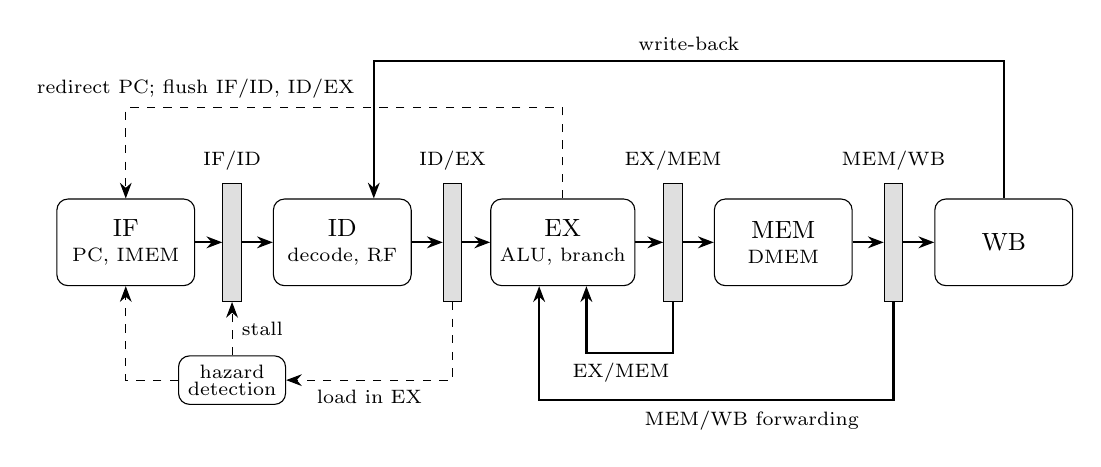
\begin{tikzpicture}[
  stage/.style={draw, rounded corners, minimum width=1.75cm, minimum height=1.1cm,
                align=center, font=\small},
  preg/.style={draw, fill=gray!25, minimum width=0.22cm, minimum height=1.5cm},
  data/.style={-{Stealth[length=2mm]}, thick},
  ctrl/.style={-{Stealth[length=2mm]}, dashed},
  lbl/.style={font=\scriptsize, align=center}
]
  \node[stage] (if)  at (0,0)     {IF\\[-2pt]\scriptsize PC, IMEM};
  \node[preg]  (r1)  at (1.35,0)  {};
  \node[stage] (id)  at (2.75,0)  {ID\\[-2pt]\scriptsize decode, RF};
  \node[preg]  (r2)  at (4.15,0)  {};
  \node[stage] (ex)  at (5.55,0)  {EX\\[-2pt]\scriptsize ALU, branch};
  \node[preg]  (r3)  at (6.95,0)  {};
  \node[stage] (mem) at (8.35,0)  {MEM\\[-2pt]\scriptsize DMEM};
  \node[preg]  (r4)  at (9.75,0)  {};
  \node[stage] (wb)  at (11.15,0) {WB};

  \node[lbl, above=1pt] at (r1.north) {IF/ID};
  \node[lbl, above=1pt] at (r2.north) {ID/EX};
  \node[lbl, above=1pt] at (r3.north) {EX/MEM};
  \node[lbl, above=1pt] at (r4.north) {MEM/WB};

  \foreach \a/\b in {if/r1, r1/id, id/r2, r2/ex, ex/r3, r3/mem, mem/r4, r4/wb}
    \draw[data] (\a) -- (\b);

  % Write-back into the register file
  \draw[data] (wb.north) -- ++(0,1.75) -| node[lbl, pos=0.25, above] {write-back}
    ([xshift=4mm]id.north);

  % Branch/jump redirect from EX
  \draw[ctrl] (ex.north) -- ++(0,1.15) -| node[lbl, pos=0.42, above]
    {redirect PC; flush IF/ID, ID/EX} (if.north);

  % Forwarding into EX
  \draw[data] (r3.south) -- ++(0,-0.65) -| node[lbl, pos=0.3, below] {EX/MEM}
    ([xshift=3mm]ex.south);
  \draw[data] (r4.south) -- ++(0,-1.25) -| node[lbl, pos=0.2, below] {MEM/WB forwarding}
    ([xshift=-3mm]ex.south);

  % Load-use hazard detection
  \node[draw, rounded corners, font=\scriptsize, align=center] (hz) at (1.35,-1.75)
    {hazard\\[-2pt]detection};
  \draw[ctrl] (r2.south) |- node[lbl, pos=0.75, below] {load in EX} (hz.east);
  \draw[ctrl] (hz.north) -- node[lbl, right] {stall} (r1.south);
  \draw[ctrl] (hz.west) -| (if.south);
\end{tikzpicture}
\caption{Pipeline overview. Solid arrows carry data; dashed arrows are hazard control.}
\label{fig:pipeline}
\end{figure}

\paragraph{Data hazards.}
A forwarding unit compares the source registers of the instruction in EX with
the destinations held in EX/MEM and MEM/WB and selects the most recent value.
The register file is write-first: an instruction in ID that reads a register
being written in WB gets the new value. Together these remove every data hazard
except load-use, which the hazard detection unit handles with one stall cycle:
the PC and IF/ID hold, and a bubble enters ID/EX.

\paragraph{Control hazards.}
Branches and jumps are resolved in EX, using the forwarded operands. A branch
decision unit evaluates all six conditions (\texttt{beq} through
\texttt{bgeu}); the target is $PC + imm$, or $(rs1 + imm)\,\&\,{\sim}1$ for
\texttt{jalr}. When the branch is taken or the instruction is a jump, the two
younger instructions are flushed, a two-cycle penalty. \texttt{jal} and
\texttt{jalr} write $PC + 4$ to \texttt{rd}, carried through the pipeline as the
instruction's result so that forwarding and write-back need no special case;
\texttt{auipc} selects the PC as ALU operand~A.

\paragraph{RV32E registers.}
Instruction fields still encode 5-bit register numbers, so
\texttt{x16}--\texttt{x31} can appear in a binary, but RV32E reserves them. With
no trap support yet, the decoder turns such an instruction into a bubble and
raises an \texttt{illegal\_reg} signal that the testbench reports.

\paragraph{Coverage.}
The core implements 31 of the 40 RV32E instructions: \texttt{lui},
\texttt{auipc}, \texttt{jal}, \texttt{jalr}, all six branches, \texttt{lw},
\texttt{sw}, the nine register-immediate and the ten register-register ALU
operations. Byte and halfword memory accesses (\texttt{lb}, \texttt{lh},
\texttt{lbu}, \texttt{lhu}, \texttt{sb}, \texttt{sh}), \texttt{fence},
\texttt{ecall} and \texttt{ebreak} are missing.

\section{Verification}

\paragraph{Unit tests.}
Twelve testbenches check individual modules (ALU, ALU control, control unit,
immediate extractor, instruction parser, register file, forwarding and hazard
units, data memory and three pipeline registers). Each prints \texttt{[PASS]} or
\texttt{[FAIL]} per check; the runner discovers them by file name and fails a
testbench with any \texttt{[FAIL]} or no checks at all.

\paragraph{Program tests.}
Fifteen assembly programs run on the whole core. Each states its expected final
state in comments, for example \texttt{\# expect: x1=7 x2=7 mem[0]=7}. Programs
are assembled with GNU \texttt{as} for \texttt{-march=rv32e}, which also rejects
\texttt{x16}--\texttt{x31}, and linked at address~0. A generic testbench loads
the program, runs until its last instruction leaves WB, and dumps registers and
memory; the runner compares the values named in the annotations. The programs
cover ALU operations, forwarding paths, load-use stalls, every branch type taken
and not taken, loops, calls and returns, \texttt{lui}/\texttt{auipc} and
assembler pseudo-instructions.

\paragraph{Pipeline trace.}
On request the testbench prints, every cycle, the instruction in each stage and
the hazard events; the runner disassembles it into a table
(Table~\ref{tab:trace}). This view shows a stall or a wrong-path instruction in
one line, where a waveform needs dozens of signals.

\begin{table}[ht]
\centering
\caption{Excerpt of the trace of the course evaluation program: a load-use stall
(cycles 4--6) and a taken branch (cycles 11--12).}
\label{tab:trace}
\scriptsize\ttfamily
\setlength{\tabcolsep}{3.5pt}
\begin{tabular}{rllllll}
\toprule
\rmfamily Cycle & \rmfamily IF & \rmfamily ID & \rmfamily EX & \rmfamily MEM & \rmfamily WB & \rmfamily Events \\
\midrule
4  & add x1,x1,x2 & add x2,x1,x0 & lw x1,4(x0)  & sw x2,4(x0)  & li x2,7      & STALL \\
5  & add x1,x1,x2 & add x2,x1,x0 & (bubble)     & lw x1,4(x0)  & sw x2,4(x0)  & \\
6  & add x1,x1,x2 & add x1,x1,x2 & add x2,x1,x0 & (bubble)     & lw x1,4(x0)  & fwdA<-WB \\
11 & sw x1,0(x0)  & add x1,x1,x1 & beq x1,x2    & sub x1,x1,x2 & sub x1,x1,x2 & FLUSH \\
12 & and x1,x1,x2 & (bubble)     & (bubble)     & beq x1,x2    & sub x1,x1,x2 & \\
\bottomrule
\end{tabular}
\end{table}

\paragraph{Simulators and lint.}
Every test runs on Icarus Verilog~13~\cite{icarus} and on Verilator~5~\cite{verilator},
and the RTL passes \texttt{verilator --lint-only -Wall}. The two simulators
disagree on what they tolerate: Verilator rejected a testbench whose ports had
gone stale, which Icarus had masked behind an earlier error.

\section{Results}

All 12 unit tests and 15 programs pass on both simulators. Table~\ref{tab:programs}
lists the programs with their retired instruction count $N$, stalls $S$ and
flushes $F$. Every cycle count equals $N + 4 + S + 2F$: four cycles to fill the
pipeline, one per load-use stall and two per taken branch or jump. The exact
match across all programs is evidence that the core stalls and flushes exactly
when it should, and never otherwise.

\begin{table}[ht]
\centering
\caption{Program tests. Cycles always equal $N + 4 + S + 2F$.}
\label{tab:programs}
\small
\begin{tabular}{llrrrr}
\toprule
Program & Exercises & $N$ & $S$ & $F$ & Cycles \\
\midrule
\texttt{3-nop}       & no hazards (NOP-separated)        & 24 & 0 & 0 & 28 \\
\texttt{arithmetic}  & same program, fewer NOPs          & 20 & 0 & 0 & 24 \\
\texttt{alu}         & register-register ALU ops         & 16 & 0 & 0 & 20 \\
\texttt{alu\_imm}    & register-immediate ALU ops        & 13 & 0 & 0 & 17 \\
\texttt{forwarding}  & back-to-back dependencies         &  7 & 0 & 0 & 11 \\
\texttt{load\_use}   & load-use stalls                   &  6 & 2 & 0 & 12 \\
\texttt{upper}       & \texttt{lui}, \texttt{auipc}      &  4 & 0 & 0 &  8 \\
\texttt{branch}      & one taken branch                  &  7 & 0 & 1 & 13 \\
\texttt{branches}    & six branch types, both outcomes   & 19 & 0 & 7 & 37 \\
\texttt{loop}        & backward branch                   & 18 & 0 & 4 & 30 \\
\texttt{jal}         & call and return                   &  6 & 0 & 3 & 16 \\
\texttt{hazards}     & load-to-branch, link forwarding   &  9 & 1 & 4 & 22 \\
\texttt{pseudo}      & assembler pseudo-instructions     & 13 & 0 & 3 & 23 \\
\texttt{evaluation}  & course evaluation program         & 12 & 1 & 1 & 19 \\
\texttt{evaluation\_preloaded} & same, data preloaded    & 10 & 1 & 1 & 17 \\
\bottomrule
\end{tabular}
\end{table}

\paragraph{Bugs found.}
The earlier version passed one of the first twelve programs. Table~\ref{tab:bugs}
lists the RTL defects that the flow above exposed. Most were silent: the design
compiled and simulated, and only produced wrong values. The first one, an
undriven wire, is reported immediately by Verilator's lint and was invisible to
Icarus.

\begin{table}[ht]
\centering
\caption{Defects in the earlier version of the core.}
\label{tab:bugs}
\small
\renewcommand{\arraystretch}{1.25}
\begin{tabular}{p{6.2cm}p{7.3cm}}
\toprule
Defect & Symptom \\
\midrule
EX/MEM forwarding read an undriven wire & forwarded operands were \texttt{z}/\texttt{x}; any back-to-back dependency failed \\
ALU control tested \texttt{funct7[6]} instead of \texttt{funct7[5]} & \texttt{sub} and \texttt{sra} executed as \texttt{add} and \texttt{srl} \\
No load-use stall (stall tied to 0) & instruction after a load used the stale value \\
Register file without write-first & a read in ID got the stale value while WB wrote the same register \\
Branch taken if \texttt{Branch} $\wedge$ \texttt{Zero}, decided in MEM & only \texttt{beq} worked; the instruction after a taken branch still executed \\
Branch offset shifted left twice, compensated in the assembler & numeric offsets doubled; binaries from standard tools ran incorrectly \\
No datapath for \texttt{jal}, \texttt{jalr}, \texttt{auipc}; \texttt{lui} decoded through \texttt{funct3} & no link register write; wrong targets and results \\
\bottomrule
\end{tabular}
\end{table}

\section{Limitations and Future Work}

The nine missing instructions are the next step: byte and halfword accesses need
byte enables and sign extension in the memory stage, and \texttt{ecall},
\texttt{ebreak} and reserved registers need a trap mechanism. Branch prediction
would remove most of the two-cycle penalty, which dominates the branch-heavy
programs in Table~\ref{tab:programs}. Finally, the core has only been simulated;
synthesis for an FPGA would show its area and maximum frequency.

\section{Conclusion}

The five-stage RV32E core described here runs all of its test programs on two
simulators, with cycle counts that match its timing model exactly. The main
lesson is methodological: the defects that stopped the first version were
simple, but they only became visible once tests stated their expected results,
the pipeline could be read cycle by cycle, and a second tool checked the RTL.

\begin{thebibliography}{9}
\bibitem{riscv-spec}
A.~Waterman and K.~Asanović (eds.).
\textit{The RISC-V Instruction Set Manual, Volume I: Unprivileged ISA}.
RISC-V International.

\bibitem{patterson}
D.~A.~Patterson and J.~L.~Hennessy.
\textit{Computer Organization and Design RISC-V Edition: The Hardware Software
Interface}. 2nd ed. Morgan Kaufmann, 2020.

\bibitem{icarus}
S.~Williams. \textit{Icarus Verilog}. \url{https://steveicarus.github.io/iverilog/}.

\bibitem{verilator}
W.~Snyder. \textit{Verilator}. \url{https://verilator.org}.
\end{thebibliography}

\end{document}
